\typeout{CVSId: $Id: prosper-doc.tex,v 1.14 2003/02/21 18:33:00 exupery Exp $}
\documentclass{article}
\def\Version{1.1}

\usepackage{color}
\usepackage{times}
\usepackage{textcomp}
\usepackage[ps2pdf,bookmarks,%
                urlcolor=blue,citecolor=blue,linkcolor=blue,%
                pagecolor=blue,%hyperindex,%
                colorlinks,hyperfigures,
           ]{hyperref}
\usepackage{index}

\makeindex

% Registered logo
\newcommand{\Registered}{\ensuremath{^{\hbox{\fontsize{5pt}{5pt}\selectfont%
      \textregistered}}}}
% Code to be put in the index
\newcommand{\code}[1]{{\bfseries\texttt{#1}}%
  \index{#1@\texttt{#1}}}
% Macro without argument
\newcommand{\codeM}[1]{{\bfseries\texttt{\textbackslash #1}}%
  \index{#1@\texttt{\textbackslash #1}}}
% Macro with argument(s)
\newcommand{\codeA}[2]{{\bfseries\texttt{\textbackslash #1%
    #2}\index{#1@\texttt{\textbackslash #1}}}}
% Code entry in the index
\newcommand{\cindex}[1]{\index{#1@\texttt{\textbackslash #1}}}

% Trademark
\newcommand{\tm}{\ensuremath{^{\hbox{\usefont{T1}{phv}{m}{n}%
        \fontsize{5pt}{5pt}\selectfont TM}}}}

\usepackage{graphicx}
\usepackage{fancybox,amssymb}
\usepackage{pstricks}

\title{Making slides in \LaTeX\ \\ with \texttt{Prosper}}
\author{\begin{tabular}{cc}
    Fr\'ed\'eric Goualard & Peter M\o{}ller Neergaard\\ 
  \textit{IRIN, Universit\'e de Nantes} & \textit{Boston University}\\
  Nantes, France & Boston, USA 
  \end{tabular}}
\date{}

\begin{document}
\maketitle
\begin{abstract}
  The \texttt{prosper} class permits producing high quality slides; it
  is also easily extendable.  This documentation is meant to be a user
  manual as well as a technical note describing how to create your own
  styles.
\end{abstract}

\section{Using the class}
%========================
\LaTeX\ files using the \texttt{prosper} class may be eventually translated
into two different formats:
\begin{itemize}
\item the Adobe\Registered\ \emph{PostScript}\tm\ format for printing
  transparencies;
\item the Adobe\Registered\ \emph{Portable Document Format} (PDF) for
  displaying slides on computers with Acrobat\Registered\ Reader in
  full-screen mode.
\end{itemize}

When translated into PDF files, \texttt{prosper} slides benefit from
additional possibilities such as transition effects between slides and
incremental display of a slide with several animation effects. The
currently supported transitions are: 
\index{transitions!supported}%
\begin{itemize}
\item \code{Split}: two lines sweep across the screen revealing the 
  new slide;
\item \code{Blinds}: multiple lines, evenly distributed across the
  screen, appear and synchronously sweep in the same direction to
  reveal the new slide;
\item \code{Box}: a box sweeps from the center, revealing the new slide;
\item \code{Wipe}: a single line sweeps across the screen from one
  edge to the other, revealing the new slide;
\item \code{Dissolve}: the old page image dissolves to reveal the new slide;
\item \code{Glitter}: similar to \texttt{Dissolve}, except the
  effect sweeps across the image in a wide band moving from one side
  of the screen to the other;
\item \code{Replace}: the effect is simply to replace the old page
  with the new page.
\end{itemize}

Figure~\ref{fig:structure} presents a bird's-eye view of the structure
of a \LaTeX\ file using the \texttt{prosper} class.


\section{Options of the class}
%=============================

The \texttt{prosper} class supports the following options (default
options are preceded by a black triangle $\blacktriangleright$, while
the others are preceded by a black square $\blacksquare$):

%--------------------------------------------------------------------- Figure -
\begin{figure}[htbp]
  \begin{center}
    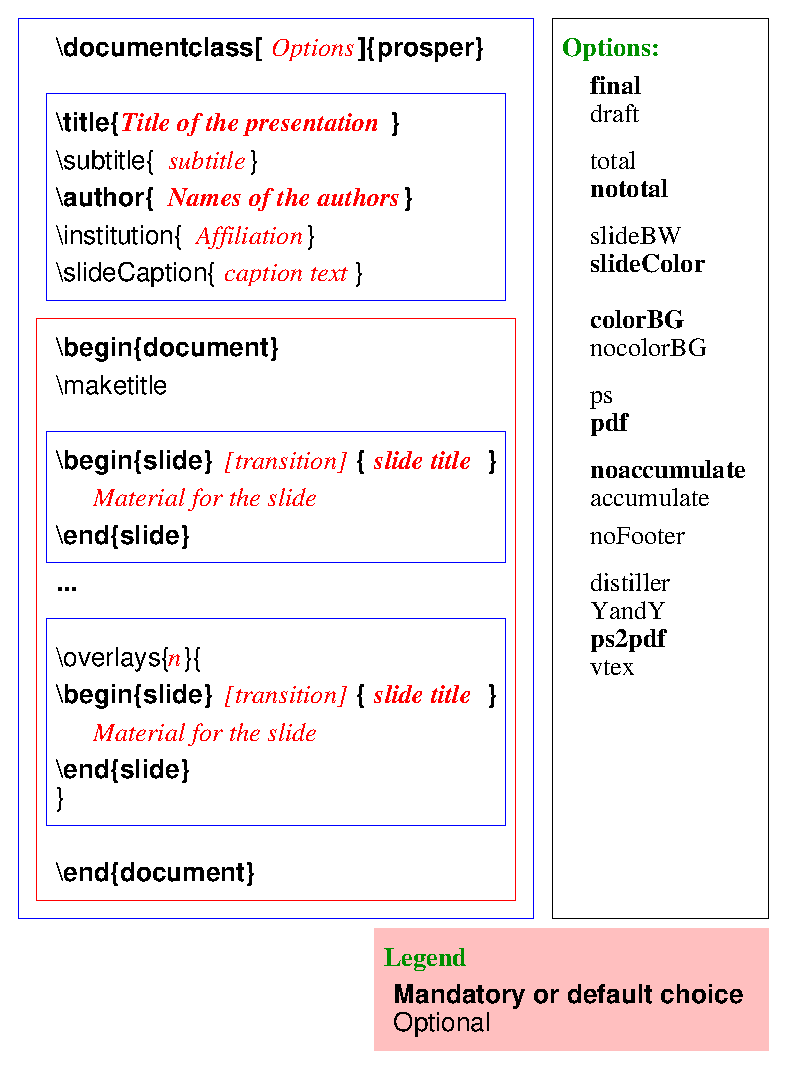
\includegraphics[width=.6\textwidth]{prosper-structure.eps}
    \caption{Structure of a \LaTeX\ file using {\normalfont\texttt{prosper}}}
    \label{fig:structure}
  \end{center}
\index{slide@\texttt{slide} environment}%
\end{figure}
%------------------------------------------------------------------------------

\begin{description}
\item [$\blacksquare$~\code{draft}.] The file is compiled in draft
  mode: figures are replaced by bounding boxes; the caption at the
  bottom of every slide displays the date and time of the compiling
  together with the file name;
\item [$\blacktriangleright$~\code{final}.] The file is compiled
  in final mode: figures are inserted at their position; the caption
  on every slide contains the text  given (optionally) by the
  user with the macro \verb$\slideCaption$, except if the
\cindex{slideCaption}%
  macro \verb$\displayVersion$ appears in the preamble (in that case,
\index{displayVersion@\texttt{\textbackslash displayVersion}}%
  the same caption as in the draft mode is used);
\item [$\blacktriangleright$~\code{slideColor}.] Slides will
  use many colors. To be used with caution when the slides are to be printed
  on a black \& white device;
\item [$\blacksquare$~\code{slideBW}.] Slides will use
  a restricted set of colors. Should be used whenever the presentation is
  meant to be printed in black \& white;
\item [$\blacksquare$~\code{total}.] The caption at the bottom of
  every slide displays the number of the current slide along with 
  the total number of slides;
\item [$\blacktriangleright$~\code{nototal}.] Only the number of the current slide
  appears in the caption;
\item [$\blacksquare$~\code{nocolorBG}.] The background of the
  slide is white whatever the style may be. It is a good idea to 
  use this option for printing slides in black \& white;
\item [$\blacktriangleright$~\code{colorBG}.] The color of
  the background depends on the current style;
\item [$\blacksquare$~\code{ps}.] The \LaTeX\ file is
  compiled to produce a PostScript\tm\ file for printing;
\item [$\blacktriangleright$~\code{pdf}.] The \LaTeX\ file is compiled to
  produce a PDF file for a presentation with a video projector;
\item [$\blacksquare$~\code{accumulate}.] Macros \verb$\onlySlide$,
\cindex{untilSlide}\cindex{fromSlide}\cindex{onlySlide}%
  \verb$\untilSlide$ and \verb$\fromSlide$ interpret their argument in
  \verb$ps$ mode. Note that it is possible to locally modify the option setting
  by using macros \codeM{Accumulatetrue} and \codeM{Accumulatefalse};
\item [$\blacktriangleright$~\code{noaccumulate}.] Macros \verb$\onlySlide$,
  \verb$\untilSlide$ and \verb$\fromSlide$ do not interpret their argument in
  \verb$ps$ mode;
\item [$\blacksquare$~\code{distiller}.] The
  PostScript\Registered\ file is to be translated into a PDF file using
  Adobe\Registered\ Distiller;
\item[$\blacksquare$~\code{YandY}.] The \LaTeX\ file is to be processed with
  YandY \LaTeX;
\item[$\blacktriangleright$~\code{ps2pdf}.] The PostScript\Registered\ 
  file is to be translated into a PDF file using AFPL \code{ps2pdf};
\item[$\blacksquare$~\code{vtex}.] The \LaTeX\ file is to be processed with MicroPress
  Visual \TeX;
\item [$\blacksquare$~\code{noFooter}.] Do not add any caption at the bottom
  of the slides.
\end{description}

\section{Predefined macros and environments} 
%===========================================

\subsection{Macros to appear in the preamble}
%--------------------------------------------
The \texttt{prosper} class (re-)defines some standard macros. Those
given hereunder are to be put in the preamble (that is, before
\index{preamble}%
\verb$\begin{document}$):

\begin{description}
\item \codeM{title}. Title of the presentation;
\item \codeM{subtitle}. Subtitle of the presentation;
\item \codeM{author}. Author(s) of the presentation;
\item \codeM{email}. E-mail address of the author(s);
\item \codeM{institution}. Name of the institute/company the author(s) 
  come(s) from;
\item \codeA{slideCaption}{\{c\}}. Caption to be put at the bottom
  of every slide (name of the event/conference\dots). 
  The title of the presentation is used as the default caption whenever 
  the author
  do not override it by providing his own caption by using this macro;
\item \codeA{Logo}{(x,y)\{mylogo\}} or \codeA{Logo}{\{mylogo\}}. 
  The logo given by \verb$mylogo$ will be put at the position \verb$(x,y)$
  on each slide (resp.\ at a default position defined by each slide style).
  The reference point is bottom left. An example of use is: \\
  \verb$\Logo(2,5){\includegraphics[width=1cm]{irinLOGO.eps}}$)
\item \codeM{displayVersion}. Displays a draft caption (with
  the name of the file, the title of the presentation, the name of the
  author(s), and the date/time of the last \LaTeX\ compiling) instead
  of the caption defined by the user even when in final mode;
\item \codeA{DefaultTransition}{\{trans\}}: definition of the default
  transition mode between slides. By default, the \texttt{Replace} mode is
\index{transition!default}%
  used;
\item \codeA{NoFrenchBabelItemize}. To be used when loading the babel 
  style with the ``french'' option in order to have the ability to choose
  ones own items. The french itemize glue is preserved;
\item \codeA{collapsedBookmarksfalse}. Since v. 2.0, all overlays have
  a bookmark. If you call this macro in the preamble, the tree of bookmarks
  is expanded, otherwise it is collapsed and only the bookmarks for the
  first slide of each overlay are visible.
\end{description}

\subsection{The \texttt{slide} environment}
%------------------------------------------
Figure~\ref{fig:structure} describes the \texttt{slide} environment. An
optional argument is the transition effect for displaying the slide. 
The default transition is \texttt{R} (Replace).

\subsection{Some \texttt{itemize} environments}
%----------------------------------------------
The \texttt{Itemize} environment corresponds to the \LaTeX\ 
\index{Itemize@\texttt{Itemize} environment}%
\texttt{itemize} environment where the text is justified. In
\index{itemize@\texttt{itemize} environment}%
\texttt{prosper}, the \texttt{itemize} environment has been redefined
such that text is not justified in it (a better choice for slides).

There also exists an \texttt{itemstep} environment where each item is displayed
\index{itemstep@\texttt{itemstep} environment}%
incrementally (in PDF mode). This environment only offers a facility
to add overlays and is quite limited in use. In particular, no nesting
of \texttt{itemstep} environment is allowed. It accepts an optional argument
corresponding to the overlay level to start from.

\subsection{Macros to be used out of any \texttt{slide} environment}
%-------------------------------------------------------------------

\begin{description}
\item \codeA{part}{[transition]\{xx\}}. Creates a slide only containing the
  text \texttt{xx} vertically and horizontally centered in the 
  font title. The transition \texttt{transition}---if given---will be used 
  for this slide.
\end{description}

\subsection{Macros that may appear in a \texttt{slide} environment}
%------------------------------------------------------------------
\begin{description}
\item \codeA{FontTitle}{\{C\}\{BW\}}. Use this macro to change the
  font/color to be used for slide titles. The first argument is for
  color slides, the second for black and white ones;
\item \codeA{FontText}{\{C\}\{BW\}}.  Use this macro to change the
  font/color to be used for slide text. The first argument is for
  color slides, the second for black and white ones;
\item \codeA{fontTitle}{\{xx\}}. Writes its argument using the
  title font and color;
\item \codeA{fontText}{\{xx\}}.  Writes its argument using the
  text font and color;
\item \codeA{ColorFoot}{\{col\}}. The footer is to be written with color
  \texttt{col};
\item \codeA{PDFtransition}{\{tr\}}. Uses \texttt{tr} as the transition
  effect from the previous slide to the current slide;
\item \codeA{myitem}{\{lvl\}\{def\}}. Defines the item of level
  \verb$lvl$ (where \verb$lvl$ may be 1, 2 or 3) to be \verb$def$. By
  default, it is a green lozenge for all levels. The following code
  define the items to be 3D bullets of different size and color (the
  corresponding PostScript\tm\ files are provided in the \texttt{img/}
  directory of the \texttt{prosper} distribution):
{\footnotesize
\begin{verbatim}
\myitem{1}{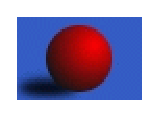
\includegraphics[width=.4cm]{red-bullet-on-blue.ps}}
\myitem{2}{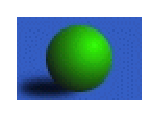
\includegraphics[width=.3cm]{green-bullet-on-blue.ps}}
\myitem{3}{
\includegraphics[width=.3cm]{yellow-bullet-on-blue.ps}}
\end{verbatim}  
}
\end{description}

\subsection{Overlays}
%--------------------

Overlays add animated effects to slides in PDF mode. They may be used
to display a slide incrementally (in several steps), for making appear and
disappear some elements on a slide\dots\ To use overlays, one has to embed
the corresponding \texttt{slide} environment into an \codeM{overlays} macro
as follows:

\begin{verbatim}
\overlays{n}{
\begin{slide}{...}
...
\end{slide}}
\end{verbatim}

The first argument (\verb$n$) of the \texttt{overlays} macro stands
for the number of steps composing the animation.

The following macros may be used to control what should appear on each
slide composing a \verb$n$ slides overlay:
\begin{itemize}
\item \codeA{fromSlide}{\{p\}\{mat\}}. Puts \verb$mat$ on slides
  \verb$p$ through \verb$n$;
\item \codeA{onlySlide}{\{p\}\{mat\}}. Puts \verb$mat$ on slide \verb$p$
  only;
\item \codeA{untilSlide}{\{p\}\{mat\}}. Puts \verb$mat$ on slides
  \verb$1$ through \verb$p$;
\item \codeA{FromSlide}{\{p\}}. All the material after the occurrence
  of the macro will be put on slides \verb$p$ through \verb$n$;
\item \codeA{OnlySlide}{\{p\}}. All the material after the occurrence
  of the macro will be put on slide \verb$p$ only;
\item \codeA{UntilSlide}{\{p\}}. All the material after the
  occurrence of the macro will be put on slides \verb$1$ through
  \verb$p$.
\end{itemize}

All those macros are only really meaningful in \verb$pdf$ mode; in
\verb$ps$ mode, they do nothing or interpret their argument, depending
on the option \verb$no/accumulate$.  Macros \verb$\fromSlide$,
\verb$\onlySlide$, and \verb$\untilSlide$ accept stared versions which
\index{fromSlide@\texttt{\textbackslash fromSlide}!stared}%
\index{onlySlide@\texttt{\textbackslash onlySlide}!stared}%
\index{untilSlide@\texttt{\textbackslash untilSlide}!stared}%
typeset the \verb$mat$ material in a zero dimension box (i.e.\ the
position pointer is not moved). The stared versions should be used for
replacement purposes. For example, the piece of code:
\begin{verbatim}
\onlySlide*{1}{\includegraphics{example-1.eps}}%
\onlySlide*{2}{\includegraphics{example-2.eps}}%
\onlySlide*{3}{\includegraphics{example-3.eps}}%
\end{verbatim}
would put image \verb$example-1.eps$ on the first slide; this image
would then be replaced by \verb$example-2.eps$ on the second slide,
and by \verb$example-3.eps$ on the third slide. Note the \verb$%$ 
comment sign at the end of each line: it prevents \LaTeX\ from inserting
some space---due to the carriage return---which would induce a slight
displacement between each image on the slides.

\medskip
\noindent\textbf{Important note}: keep in mind that 
\verb$\FromSlide$, 
\verb$\OnlySlide$, \verb$\UntilSlide$, and the un-stared versions of
\verb$\fromSlide$, \verb$\onlySlide$, and \verb$\untilSlide$ interpret
the argument \verb$mat$ \emph{for each slide composing the overlay}
even if it is not displayed (this is mandatory in order to know the size of the
box that needs be reserved for the un-displayed material).

The following macros permit choosing the material to put on a slide depending 
on the chosen mode (ps or pdf):
\begin{itemize}
\item \codeA{PDForPS}{\{ifpdf\}\{ifps\}}. Interprets material \verb$ifpdf$ 
  if the chosen mode is \verb$pdf$, otherwise interprets \verb$ifps$;
\item \codeA{onlyInPS}{\{mat\}}. Interprets material \verb$mat$ only if
  the mode is \verb$ps$;
\item \codeA{onlyInPDF}{\{mat\}}. Interprets material \verb$mat$ only if
  the mode is \verb$pdf$.
\end{itemize}

These macros may be used as follows:
\begin{verbatim}
\overlays{3}{%
\begin{slide}{Example}
\onlySlide*{1}{\includegraphics{example-1.eps}}%
\onlySlide*{2}{\includegraphics{example-2.eps}}%
\onlySlide*{3}{\includegraphics{example-3.eps}}%
\onlyInPS{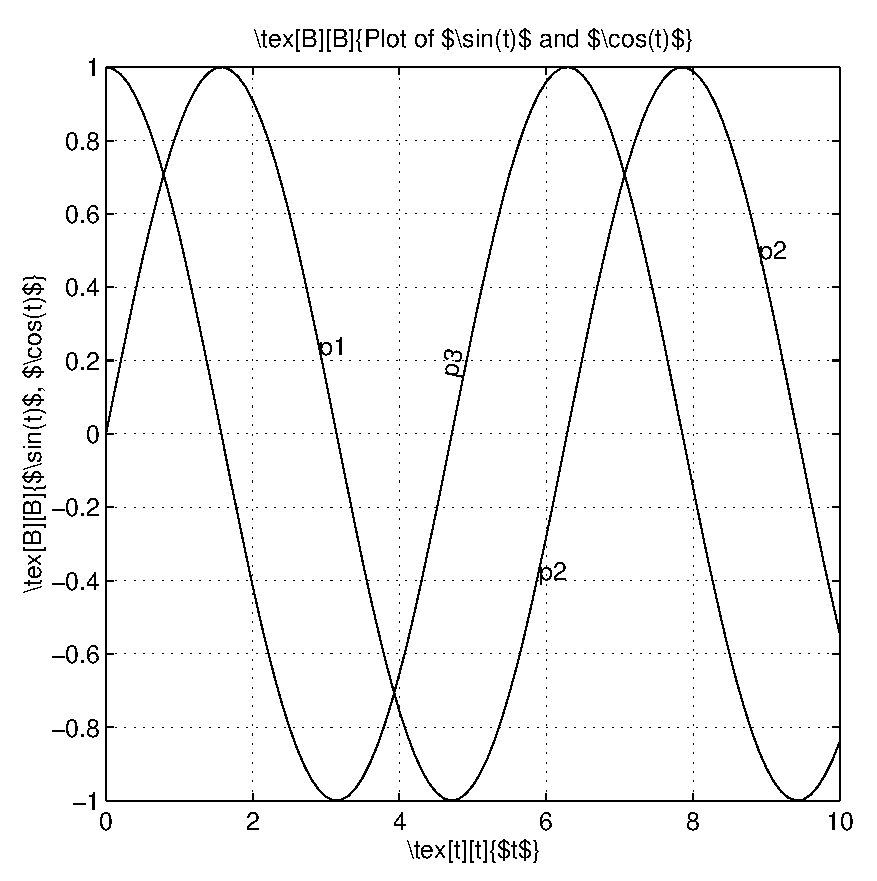
\includegraphics{example.eps}}%
\end{slide}}
\end{verbatim}
This slide will be displayed in three steps with three different
figures in \verb$pdf$ mode; in \verb$ps$ mode, there will be only one
slide containing figure \verb$example.eps$.

\section{Warning}\label{sec:avertissement}
%=================

The \texttt{prosper} slide styles are not bound to provide the same
display area. Consequently, using different styles may require some
\index{slide!display area}%
adjustment in the text and graphics positioning.

\section{The Compilation Process}
%================================

The compilation process slightly differs depending on the intended use of
the slides. It is sketched in Fig.~\ref{fig:compilation}. If you plan
to print slides on transparencies, you should select the \verb$ps$
option and create a PostScript\tm\ file, while if you want to display them
with a computer and an overhead projector, you should select the
\verb$pdf$ option and create a PDF file from the PostScript\tm\ file.
Translation of a PostScript\tm\ file into a PDF file is done by the
program \texttt{ps2pdf} included in the GhostScript distribution.

%--------------------------------------------------------------------- FIGURE -
\begin{figure}[htbp]
  \begin{center}
    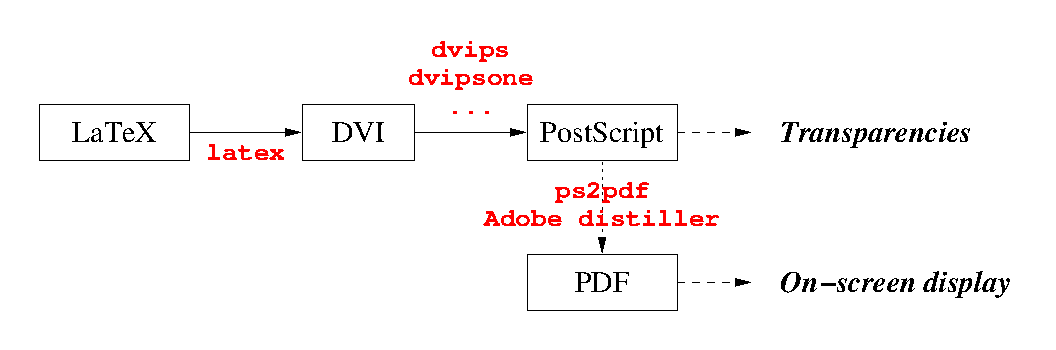
\includegraphics[width=\textwidth]{compilation.eps}
    \caption{Compilation process}
    \label{fig:compilation}
  \end{center}
\end{figure}
%------------------------------------------------------------------------------

\noindent\textbf{Important note}: PDF file should be made resolution 
independent by using vectorial fonts only (no \TeX\ bitmap fonts). To
do so, you have to use a GhostScript version at least equal to 6.0.
You also need to create a \verb$.dvipsrc$ file in your home directory
with the following lines:
\begin{verbatim}
p +psfonts.cmz
p +psfonts.amz
\end{verbatim}
Last, \texttt{prosper} styles have been devised to be used with A4 European
paper format. Consequently, you will have to instruct GhostScript to
use the appropriate format by defining the \code{GS\_OPTIONS}
environment variable to \verb$"-sPAPERSIZE=a4"$. If you use bash as
\cindex{PAPERSIZE}%
your main shell, this is done by adding the line
\begin{verbatim}
export GS_OPTIONS="-sPAPERSIZE=a4"
\end{verbatim}
in your \verb$.bash_profile$ file.

You will need Adobe\Registered\ Acrobat\Registered\ Reader
(\texttt{acroread}) to display PDF files. It is available for free on
the Adobe\Registered\ \href{http://www.adobe.com/}{web site}.
Acrobat\Registered\ Reader provides a full-screen mode that is
particularly handy for presentations.

\section{Devising new slide styles}
%===================================

Devising new \texttt{prosper} styles is an easy task provided you know
the basics of Van Zandt's \texttt{PSTricks} package (refer to
\emph{PSTricks: PostScript\tm\ macros for Generic \TeX}, User's Guide,
Timothy Van Zandt).  In order to devise your own style named
\texttt{foo}, you first have to create a file
\texttt{PPR\textbf{foo}.sty} which will contain its definition. Refer
to predefined styles for some examples and to
Section~\ref{sec:definition-example}.

\noindent\textbf{A word of caution:} you are free to create a new 
style by modifying an existing one. In that case, \textbf{it is
  MANDATORY} renaming your file; do NEVER EVER modify a style without
renaming it (is that clear enough?).  You should also write your name
and email address in any of your styles such that users know who to
get in touch with when they use the style. Please choose a name for
your style that is unique in the \texttt{prosper} distribution (with
respect to both predefined and contributed styles so far).

\medskip Please send slide styles you are proud of. I will add them to
the distribution in the \texttt{contrib/} directory. Note that I will
only consider for addition styles that are indeed original. Modifying
the colors or the fonts of an existing one is definitely not
sufficient since this can be done by users in their \LaTeX\ file by using
the provided hooks for customization.

\subsection{Predefined tests}
%-----------------------------
The following tests may be used in your style file in order to modify
its behaviour according to the active options. The general scheme is:
\begin{verbatim}
       \ifxxxx%
           % The ``then'' part
       \else%
           % The ``else'' part
       \fi
\end{verbatim}

\begin{description}
\item \codeM{ifDVItoPS}. True when the DVI file will be eventually 
  translated into a PostScript\tm\ file, false when the final target is
  the PDF format;
\item \codeM{ifisDraft}. True when the file is compiled in draft mode;
\item \codeM{ifinColor}. True when the option \texttt{slideColor} 
  has been chosen;
\item \codeM{ifallPages}. True when the option \texttt{total} has
  been chosen;
\item \codeM{ifcolorBG}. True when the option \texttt{colorBG} has
  been chosen;
\item \codeM{ifshowVersion}. True whenever the macro 
  \verb$\displayVersion$ appears in the preamble;
\item \codeM{ifInOverlays}. True if the current \texttt{slide} 
  environment is embedded into an \texttt{overlays} macro.
\end{description}

\subsection{Macros to customize or create a style}
%-------------------------------------------------
\begin{description}
\item \codeA{slideCaption}{\{cap\}}. Definition of a caption
  to appear on every slide;
\item \codeA{PDFCroppingBox}{\{lx ly ux uy\}}. Definition of a
  PostScript\tm\ \emph{bounding box} to crop slides for enhancing
\index{bounding box}%
  their appearance on $4/3$ devices such as monitors (only used in PDF
  mode);
\item \codeA{NewSlideStyle}{[width]\{anchor\}\{pos\}\{defin\}}.
  Defines a new slide style whose definition is given by the macro
  \verb$\defin$ and whose contents area has width \verb$width$ and is
  put at position \verb$(pos)$ with anchor \verb$anchor$. If no width
  is given, a default width of 11\,cm is used;
\item \codeA{LogoPosition}{\{pos\}}. Default position for a logo if none
  is given by the user;
\item \codeM{PutLogo}. A macro to be put at the end of the macro
  that defines your own style.
\end{description}

\subsection{Lengths}
%-------------------

\begin{description}
\item \codeM{slideWidth}. Defines the width of the text area in the slide. 
  Should not be modified by the user. Corresponds to the first argument of
  macro \code{NewSlideStyle}.
\end{description}

\subsection{Example: the \texttt{troispoints} style}
%----------------------------------------------------
\label{sec:definition-example}

\begin{small}
\begin{verbatim}
\NeedsTeXFormat{LaTeX2e}[1995/12/01]
\ProvidesPackage{PPRtroispoints}[2000/04/17]
\typeout{`Trois points' style for Prosper ---}
\typeout{(c) 2000 Frederic Goualard, CWI, The Netherlands}
\typeout{CVSId: $Id: prosper-doc.tex,v 1.14 2003/02/21 18:33:00 exupery Exp $}
\typeout{ }

\RequirePackage{amssymb}
% Loading packages necessary to define this slide style.
\IfFileExists{pst-grad}{\RequirePackage{pst-grad}}{\RequirePackage{gradient}}

\newgray{mygrey}{.5}
\newrgbcolor{mellow}{.847 .72 .525}
\newrgbcolor{orange}{1.00 0.65 0.00}

\FontTitle{%
  \usefont{T1}{ptm}{m}{sl}\fontsize{22pt}{20pt}\selectfont\orange}{%
  \usefont{T1}{ptm}{m}{sl}\fontsize{22pt}{20pt}\selectfont\blue}
\FontText{%
  \mellow\usefont{T1}{phv}{m}{n}\fontsize{14.4pt}{14pt}\selectfont}{%
  \black\usefont{T1}{phv}{m}{n}\fontsize{14.4pt}{14pt}\selectfont}

\ColorFoot{\mellow}

% Positionning of the title of a slide.
\newcommand{\slidetitle}[1]{%
  \rput[l](-0.4,3.7){\parbox{10cm}{\fontTitle{#1}}}
}

% Positionning for a logo
\LogoPosition{-1,-1.1}

% Definition of this style for slides.

\newcommand{\TPFrame}[1]{%
  \ifinColor
  \ifcolorBG
  \psframe[linestyle=none,fillstyle=solid,fillcolor=black](-2,-1.4)(12.5,9)
  \fi
  \fi
  \psframe[linestyle=dotted,dotsep=5pt,linewidth=2pt,linecolor=mellow]%
  (-1,-.5)(11.6,8.3)
  \pspolygon[linestyle=none,fillstyle=solid,%
  fillcolor=mygrey](8.4,8.4)(9.6,8.4)(9,7.4)
  \pspolygon[linestyle=none,fillstyle=solid,%
  fillcolor=red](8.2,8.5)(9.4,8.5)(8.8,7.5)
  \pspolygon[linestyle=none,fillstyle=solid,%
  fillcolor=mygrey](1.4,-1.1)(2.6,-1.1)(2,-.1)
  \pspolygon[linestyle=none,fillstyle=solid,%
  fillcolor=red](1.1,-.9)(2.3,-.9)(1.7,.1)
  \PutLogo % Mandatory
 {#1}}

\NewSlideStyle{t}{5.3,2.9}{TPFrame}
\PDFCroppingBox{10 40 594 800}
\RequirePackage{semhelv}

\endinput
\end{verbatim}
\end{small}


\section{Copyright information}
%===============================
Copyright \copyright{} 2000-2003 by Fr\'ed\'eric Goualard and Peter M�ller Neergaard, all rights reserved.
 
\medskip\noindent
This program may be distributed and/or modified under the
conditions of the LaTeX Project Public License, either version 1.2
of this license or (at your option) any later version.
The latest version of this license is in
\href{http://www.latex-project.org/lppl.txt}{http://www.latex-project.org/lppl.txt} and version 1.2 or later is part of all distributions of LaTeX 
version 1999/12/01 or later.

\section{The Prosper homepage}
%=============================

The official Prosper homepage is located at Source Forge (tm):

\begin{center}
\texttt{\href{http://prosper.sourceforge.net/}{http://prosper.sourceforge.net/}}
\end{center}

You will find there additional information, CVS tarballs, news, up to
date distributions of Prosper\dots\ If you plan using Prosper on a
regular basis, you should consider subscribing to the lists
\texttt{prosper-users} and \texttt{prosper-announce}.  Directions to
subscribe to them are available on the homepage.



\section{Troubleshootings}
%=========================

If you experience some problem when installing or using Prosper,
please go first to the Prosper homepage to check whether there is some
hint on how to solve it in one of the list archives. If you do not
find any answer to your problem, send a mail to the
\texttt{prosper-users} list.

Mails asking for help sent directly to the authors will \emph{not} be
taken into consideration.

There is also a file \texttt{TROUBLESHOOTINGS} in the distribution listing
solutions to commonly encountered problems.

Prosper relies on some recent versions of some packages and software
(mainly \texttt{hyperref} and Aladdin GhostScript). Check the homepage
to find links to the required versions.

\section{Bugs reports}
%=====================

Bugs are to be reported by filling the appropriate forms available at
the Prosper homepage. 

\section{Contributors}
%%====================

AVK provided the patchs to support MicroPress VTeX.


\printindex
\end{document}

%%% Local Variables: 
%%% mode: latex
%%% TeX-master: t
%%% End: 
